\section{Erreurs de dimension}

Si vous n'êtes pas satisfait de la précision dimensionnelle de vos impressions, vérifiez d'abord que votre microprogramme est correctement configuré: les échelons / millimètres pour les axes X, Y et Z doivent être calculés en fonction de vos courroies, poulies et vis filetées. Veuillez ne pas calibrer par essai et erreur: ces valeurs doivent être exactes. Utilisez la calculatrice de Josef Prusa\footnote{\url{http://www.prusaprinters.org/calculator/}}.

\subsection{Dimensions verticales}

Si vos dimensions verticales sont fausses (c'est-à-dire le long de l'axe Z) - et votre objet est généralement plus court que prévu - cela signifie que votre buse est trop basse, donc la première couche est trop pressée sur le lit d'impression. Pour résoudre ce problème, vous voudrez peut-être augmenter votre Z-endstop ou augmenter l'option de décalage Z dans Slic3r.

\subsection{Dimensions horizontales}

Le problème habituel est que les trous sont trop petits. Cela affecte habituellement uniquement les trous sur le plan horizontal (XY). Il y a plusieurs raisons à cela. Voyons les voir un par un:

\subsection{Rétrécissement du plastique}

Le plastique \textbf{rétrécit lors du refroidissement}. Différents types de plastique présentent un retrait différent, qui peut également dépendre de la température. Du fait de ce retrait, des trous circulaires (ou polygonaux) posés par l'extrudeuse au diamètre nominal finiront par diminuer après refroidissement.

\subsection{Plus de matière déposé à l'interieur}

Lorsque vous extrudez le long d'une courbe, plus de matériau par unité de distance est déposé dans le côté concave. Un tel matériau excessif rend le rayon interne plus court. Un algorithme de compensation a été proposé par Adrian Bowyer et il a été implémenté dans Slic3r il ya quelque temps, mais de nombreux utilisateurs se sont plaints de trous trop grands - il a été enlevé par la suite depuis plus petits trous sont meilleurs que les trous plus grands car ils peuvent être forés.

\subsection{Les courbes sont approximées par des polygones}

Les fichiers STL ne contiennent que des mailles composées de triangles plats, de sorte que ses sections planes ne peuvent contenir que des formes polygonales. Par exemple, un trou circulaire est approximé par un polygone:

\begin{figure}[H]
\centering
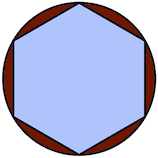
\includegraphics[keepaspectratio=true,width=0.3\textwidth]{troubleshooting/polygonal-hole.png}
\caption{Trou en forme de polygone}
\label{fig:polygonal-hole}
\end{figure}
Augmenter le nombre de segments dans votre CAO avant d'exporter le fichier STL aidera à réduire l'erreur. Les utilisateurs d'OpenSCAD peuvent vouloir utiliser la fonction polyhole () développée par nophead qui calcule le nombre optimal de segments.

\subsection{Le filament tend à couper les coins}

Puisque les courbes sont approximées par des polygones, il y a des sommets tranchants à leurs sommets. Cependant, le plastique tend à faire des coins arrondis, réduisant ainsi la zone interne du trou encore plus.

\subsection{Ondulation verticale}

Même si la précision dimensionnelle d'une seule couche était correcte, plusieurs couches empilées pourraient rendre le trou plus petit si elles ne sont pas exactement alignées. Les ondulation verticale (\ref{sec:z_wobble}) causée par des problèmes mécaniques réduira la taille des trous à l'enveloppe interne des couches empilées:

\begin{figure}[H]
\centering
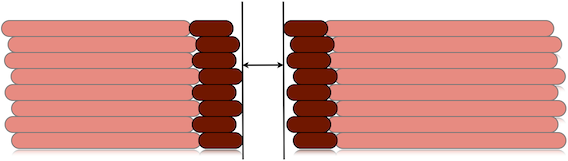
\includegraphics[keepaspectratio=true,width=1\textwidth]{troubleshooting/z-wobble.png}
\caption{Ondulation verticale}
\label{fig:z_wobble}
\end{figure}

\subsection{Filament irrégulier}

Les filaments de qualité médiocre et de faible qualité n'ont pas un diamètre très régulier. Si vous mesurez leur diamètre le long d'un seul mètre d'entre eux, vous trouverez souvent de nombreuses valeurs différentes (et de nombreux filaments de mauvaise qualité et n'ont pas de section parfaitement ronde). Cette variation continue de diamètre produira un écoulement irrégulier et le trou résultant sera toujours l'enveloppe interne de toutes les couches:

\begin{figure}[H]
\centering
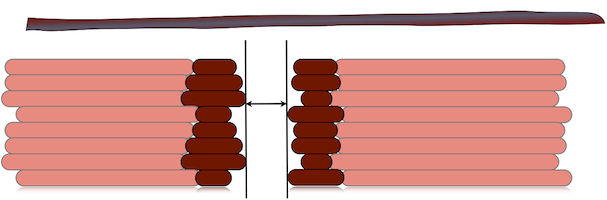
\includegraphics[keepaspectratio=true,width=1\textwidth]{troubleshooting/irregular-filament.png}
\caption{Filament irrégulier}
\label{fig:irregular_filament}
\end{figure}

\subsection{Contrecoup}

Le jeu est un défaut mécanique d'un ou plusieurs axes qui réduit essentiellement la quantité de mouvement réel chaque fois qu'un moteur inverse sa direction de rotation. Il est généralement causé par des ceintures lâches. Sur les imprimantes à lit mobile, son axe (habituellement Y) est plus sujet à un jeu à cause de l'inertie. Donc, si vous obtenez des erreurs de dimension différentes dans X et Y, cela est causé par le jeu. Vous aurez besoin de serrer votre ceinture. Aucun hack logiciel ne peut raisonnablement compenser une imprimante mal assemblée.

\subsection{Calcul de flux}

Bon, toutes les causes ci-dessus ne dépendent pas de Slic3r et, quand cela est possible, ils doivent être corrigés avant de tenter une solution logicielle.

Cela dit, les calculs de flux utilisés dans Slic3r jouent un bon rôle dans la prise des dimensions correctes, car il essaie de deviner quelle est la forme du matériau extrudé sera et comment l'épaisseur de l'extrusion résultera sur le plan horizontal donné une quantité de matériau. Étant une approximation, elle porte une erreur. La façon habituelle de traiter ces questions implique de régler le paramètre Extrusion Multiplier afin d'augmenter / réduire la quantité de plastique, ce qui rend les extrusions plus ou moins épaisses. Mais cela affectera également les surfaces solides, ce n'est donc pas la solution idéale.

Pour des dimensions plus exactes, vous devez vérifier l'option \textbf{External Perimeters First}. L'impression des périmètres extérieurs empêchera d'abord le déplacement provoqué par le chevauchement de l'extrudat. D'autre part, l'impression des périmètres internes couvre d'abord les coutures mieux, donc c'est votre prise.

Une nouvelle option \textbf{XY size Compensation} à également été introduite qui permet de faire croître / rétrécir la forme de l'objet afin de compenser l'erreur mesurée. Supposons que vos trous soient plus petits de 0.1mm, vous pouvez simplement entrer -0.05 dans cette option pour les obtenir compensés (signe négatif signifie rétrécissement vers l'intérieur).
